\documentclass[a4paper,onecolumn,oneside,12pt,extrafontsizes]{memoir}


\usepackage[T1]{fontenc}
\usepackage[polish]{babel}
\usepackage[utf8]{inputenc}
\usepackage{setspace}
\usepackage{tabularx}
\usepackage{color,calc}
\selectlanguage{polish}
\usepackage{lmodern}
\usepackage{graphicx}
\usepackage{titlesec}
\setcounter{secnumdepth}{4}
\usepackage{caption}
\usepackage{graphicx}
%\usepackage{picture}
%\usepackage{gensymb}
%\usepackage{listingsutf8}
%\lstset{language=Pascal}
%\usepackage{listings}

\usepackage{ebgaramond}

\usepackage{tgtermes}

\usepackage{amsmath}  
\usepackage{fixltx2e} 


\clubpenalty=10000      %kara za sierotki
\widowpenalty=10000  % nie pozostawiaj wdów
\brokenpenalty=10000		% nie dziel wyrazów między stronami
\exhyphenpenalty=999999		% nie dziel słów z myślnikiem
\righthyphenmin=6			% dziel minimum 3 litery

\renewcommand{\topfraction}{0.95}
\renewcommand{\bottomfraction}{0.95}
\renewcommand{\textfraction}{0.05}
\renewcommand{\floatpagefraction}{0.35}

\setlength{\headsep}{10pt} 
\setlength{\headheight}{13.6pt}
\setlength{\footskip}{\headsep+\headheight}
\setlength{\uppermargin}{\headheight+\headsep+1cm}
\setlength{\textheight}{\paperheight-\uppermargin-\footskip-1.5cm}
\setlength{\textwidth}{\paperwidth-5cm}
\setlength{\spinemargin}{2.5cm}
\setlength{\foremargin}{2.5cm}
\setlength{\marginparsep}{2mm}
\setlength{\marginparwidth}{2.3mm}
\checkandfixthelayout[fixed]

%\linespread{1}
\linespread{1.3}
\setlength{\parindent}{14.5pt}


\makeatletter
\newcommand{\showFontSize}{\f@size pt} % makro wypisujące wielkość bieżącej czcionki
\makeatother


\captionnamefont{\small}
\captiontitlefont{\small}
%%%%%%%%%%%%%%%%%%%%%%%%%%%%%%%%%%%%%%%
%% Definicja strony tytułowej 
%%%%%%%%%%%%%%%%%%%%%%%%%%%%%%%%%%%%%%%
\makeatletter
%Uczelnia
\newcommand\uczelnia[1]{\renewcommand\@uczelnia{#1}}
\newcommand\@uczelnia{}
%Wydział
\newcommand\wydzial[1]{\renewcommand\@wydzial{#1}}
\newcommand\@wydzial{}
%Kierunek
\newcommand\kierunek[1]{\renewcommand\@kierunek{#1}}
\newcommand\@kierunek{}
%Specjalność
\newcommand\specjalnosc[1]{\renewcommand\@specjalnosc{#1}}
\newcommand\@specjalnosc{}
%Tytuł po angielsku
\newcommand\titleEN[1]{\renewcommand\@titleEN{#1}}
\newcommand\@titleEN{}
%Tytuł krótki
\newcommand\titleShort[1]{\renewcommand\@titleShort{#1}}
\newcommand\@titleShort{}
%Promotor
\newcommand\promotor[1]{\renewcommand\@promotor{#1}}
\newcommand\@promotor{}

\usepackage[absolute]{textpos} % zamarkowano, bo ostatecznie wykorzystano otoczenie picture

\def\maketitle{%
	\pagestyle{empty}%
	%%\garamond 
	\fontfamily{\ebgaramond@family}\selectfont % na stronie tytułowej czcionka garamond
	%%%%%%%%%%%%%%%%%%%%%%%%%%%%%%%%%%%%%	
	%% Poniżej, w otoczniu picture, wstawiono tytuł i autora. 
	%% Tytuł (z autorem) musi znaleźć się w obszarze 
	%% odpowiadającym okienku 110mmx75mm, którego lewy górny róg 
	%% jest w położeniu 77mm od lewej i 111mm od górnej  krawędzi strony 
	%% (tak wynika z wycięcia na okładce). 
	%% Poniższy kod musi być użyty dokładnie w miejscu gdzie jest.
	%% Jeśli tytuł nie mieści się w okienku, to należy tak pozmieniać 
	%% parametry użytych komend, aby ten przydługi tytuł jednak 
	%% upakować go do okienka.
	%%
	%% Sama okładka (kolorowa strona z wycięciem, do pobrania z dydaktyki) 
	%% powinna być przycięta o 3mm od każdej z krawędzi.
	%% Te 3mm pewnie zostawiono na ewentualne spady czy też specjalną oprawę.
	%%%%%%%%%%%%%%%%%%%%%%%%%%%%%%%%%%%%%	
	\newlength{\tmpfboxrule}
	\setlength{\tmpfboxrule}{\fboxrule}
	\setlength{\fboxsep}{2mm}
	\setlength{\fboxrule}{0mm} 
	%\setlength{\fboxrule}{0.1mm} %% jeśli chcemy zobaczyć ramkę
	\setlength{\unitlength}{1mm}
	\begin{picture}(0,0)
	\put(26,-124){\fbox{
			\parbox[c][71mm][c]{104mm}{\centering 
				{\fontsize{16pt}{18pt}\selectfont \@title}\\[5mm]
				{\fontsize{16pt}{18pt}\selectfont \@titleEN}\\[20mm]
				{\fontsize{16pt}{18pt}\selectfont AUTOR:}\\[2mm]
				{\fontsize{14pt}{16pt}\selectfont \@author}}
		}
	}
	\end{picture}
	\setlength{\fboxrule}{\tmpfboxrule} 
	%%%%%%%%%%%%%%%%%%%%%%%%%%%%%%%%%%%%%
	%% Reszta strony z nazwą uczelni, wydziału, kierunkiem, specjalnością
	%% promotorem, oceną pracy, miastem i rokiem
	{\centering%\vspace{-1cm}
		{\fontsize{22pt}{24pt}\selectfont \@uczelnia}\\[0.4cm]
		{\fontsize{22pt}{24pt}\selectfont \@wydzial}\\[0.5cm]
		\hrule %\vspace*{0.7cm}
	}
	{\flushleft\fontsize{14pt}{16pt}\selectfont%
		\begin{tabular}{ll}
			KIERUNEK: & \@kierunek\\
			SPECJALNOŚĆ: & \@specjalnosc\\
		\end{tabular}\\[1.3cm]
	}
	{\centering
		{\fontsize{32pt}{36pt}\selectfont PRACA DYPLOMOWA}\\[0.5cm]
		{\fontsize{32pt}{36pt}\selectfont MAGISTERSKA}\\[2.5cm]
	}
	\vfill
	

	\begin{tabularx}{\linewidth}{p{6cm}l}
		&{\fontsize{16pt}{18pt}\selectfont PROWADZĄCY PRACĘ:}\\[2mm] %UWAGA: tutaj jest miejsce na nazwisko promotora pracy
		&{\fontsize{14pt}{16pt}\selectfont \@promotor}\\[10mm]
		&{\fontsize{16pt}{18pt}\selectfont OCENA PRACY:}\\[20mm]
	\end{tabularx}

	\vspace{2cm}
	\hrule\vspace*{0.3cm}
	{\centering
		{\fontsize{16pt}{18pt}\selectfont \@date}\\[0cm]
	}
	%\ungaramond
	\normalfont
	\cleardoublepage
}
\makeatother


%%%%%%%%%%%%%%%%%%%%%%%%%%%%%%%%%%%%%%%%%
%%  Metadane dokumentu 
%%%%%%%%%%%%%%%%%%%%%%%%%%%%%%%%%%%%%%%%%
\title{Filtry cząsteczkowe i ich zastosowania w problemach wyznaczania lokalizacji}
\titleEN{Particle filters for selected problems in positioning}
\author{inż. Wojciech Sopot}
\uczelnia{POLITECHNIKA WROCŁAWSKA}
\wydzial{WYDZIAŁ ELEKTRONIKI}
\kierunek{AUTOMATYKA I ROBOTYKA}
\specjalnosc{SYSTEMY INFORMATYCZNE W AUTOMATYCE}
\promotor{dr hab. inż. Paweł Wachel, K$28$W$04$}
\date{WROCŁAW, 2021}


% moje libki start

\usepackage{tikz-cd}
\usepackage{enumitem}

\usepackage[ruled,vlined]{algorithm2e}
%\usepackage[ruled]{algorithm2e}
\renewcommand{\algorithmcfname}{Algorytm}

\setcounter{secnumdepth}{5}
\setcounter{tocdepth}{5}
\usepackage{float}
% moje libki end
\begin{document}
	\maketitle
	\pagestyle{plain}
	\tableofcontents	
	\chapter{Wprowadzenie}
W rozdziale przedstawiono cel i zakres pracy oraz podstawowe zadania i problemy wyznaczania lokalizacji. Ponadto opisano ogólną ideę stojącą za filtrami cząsteczkowymi - filtrację bayesowską. 
\section{Zadania i problemy wyznaczania lokalizacji}
Mogłoby się wydawać, iż w dzisiejszych czasach, gdy mamy możliwość korzystania z systemu GPS, nie ma potrzeby zajmować się innymi sposobami wyznaczania lokalizacji. Jednak o ile jest to prawdą w dużej skali, jak np. gdy chce się wyznaczyć adres w mieście pod którym się znajdujemy, to gdy chcemy wyznaczyć swoją lokalizację bardziej dokładnie, np. jak to robią niektóre odkurzacze mobilne, to trzeba wykorzystać do tego dane z innych sensorów, np. lidarów. Czasami można wcale nie mieć możliwości korzystania z systemu GPS, na przykład pod wodą. Innym problemem może być poprawa już znanego przybliżonego położenia. W pracy zostaną przeanalizowane dwa problemy związane z wyznaczaniem lokalizacji:
\begin{itemize}
	\item Określanie położenia samolotu, na podstawie znanej mapy wysokościowej terenu, odczytów z wysokościomierza barometrycznego, oraz, ewentualnie, dodatkowych danych (np. odczytu z kompasu). 
	\item Określanie lokalizacji robota mobilnego, umieszczonego w ograniczonej przestrzeni z przeszkodami (ale na płaskiej powierzchni - mapa jest w dwóch wymiarach).
\end{itemize}
Mimo tego, iż są to jedynie dwa przypadki, w praktyce można je uogólnić na wiele sytuacji. Dla przykładu w \cite{underwater_pf} zajęto się problemem lokalizacji pod wodą, który w praktyce można rozwiązać w ten sam sposób co problem samolotu - mapa wysokości zostaje jedynie zastąpiona przez mapę głębokości.
\section{Cel pracy}
Celem pracy jest rozpoznanie możliwości zastosowania filtrów cząsteczkowych do rozwiązywania problemu lokalizacji oraz samodzielne zaimplementowanie i przebadanie kilku, uznanych arbitralnie przez autora za najciekawsze.
\section{Zakres pracy}
W zakres pracy wchodzi przegląd literatury na temat filtrów cząsteczkowych pod kątem problemów wyznaczania lokalizacji, następnie wybranie kilku rozwiązań oraz ich przebadanie. Aby było to możliwe konieczny jest także przegląd znanych narzędzi programistycznych, które mogą być zastosowane do zaimplementowania algorytmów.

\section{Idea filtracji Bayesowskiej}
Na chwilę obecną, algorytmy oparte o filtrację Bayesowską są szeroko wykorzystywane w automatyce i robotyce. W skrócie, podejście to polega na przeprowadzaniu cykli predykcji i poprawek, na podstawie rozkładu a priori oraz zbieranych w kolejnych iteracjach pomiarów, w celu wyznaczenia rozkładu a posteriori stanu systemu. Ideę tego podejścia widać na rysunku \ref{bayes_fil_idea}. 
\begin{figure}[H]
	\begin{center}
		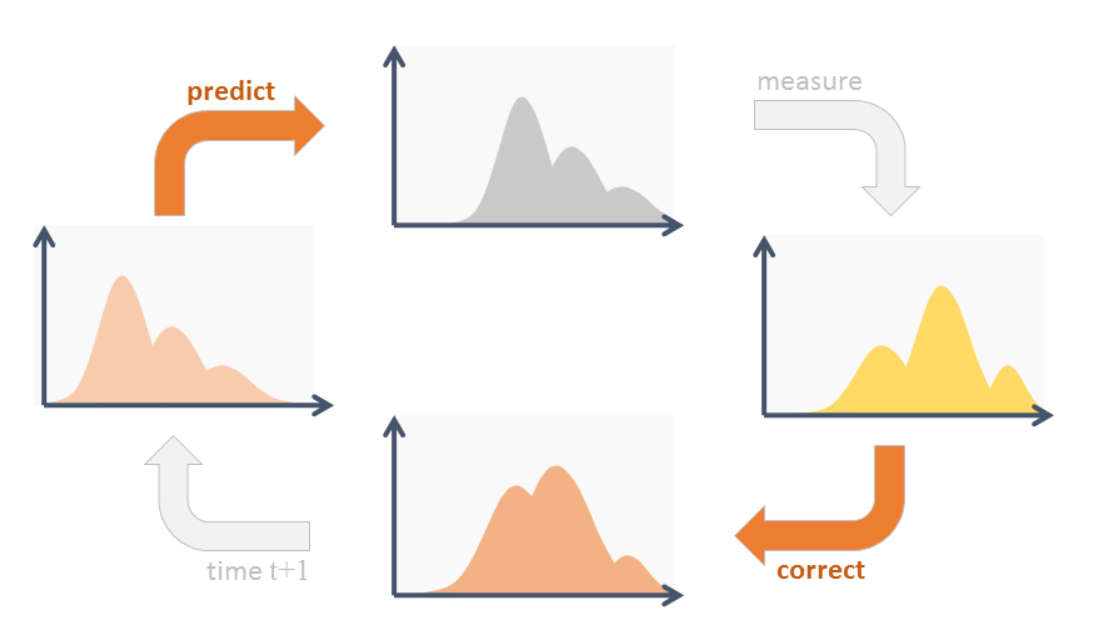
\includegraphics[width=10cm]{./predict_update.png}
		\caption{Idea filtracji Bayesowskiej. Obrazek zaczerpnięto z https://www.codeproject.com/Articles/865934/Object-Tracking-Particle-Filter-with-Ease}
		\label{bayes_fil_idea}
	\end{center}
\end{figure}
Na rysunku \ref{filtr_hier} przedstawiono hierarchię rozwiązać opartych o to podejście. Jak widać jest to bardzo duża rodzina rozwiązań, jednak w pracy zostaną poruszone jedynie metody oparte o filtry cząsteczkowe.
\begin{figure}[H]
	\begin{center}
		\includegraphics[width=10cm]{./nfg001.jpg}
		\caption{Hierarchia filtrów opartych o filtrację Bayesowską. Obrazek zaczerpnięto z \cite{prac_gui}} \label{filtr_hier}
	\end{center}
\end{figure}

	\include{filtry_cząsteczkowe}
	\include{wybrane_narzędzia_programistyczne}
	\chapter{Badania} \label{przeg}
W tym rozdziale opisano przeprowadzone na kodzie badania. Zaczęto od opisania konkretnych problemów którymi się zajmowano, a następnie przeprowadzono badania mające potwierdzić czy algorytmy działają poprawnie. Na koniec przebadano zachowanie zaimplementowane filtry pod różnymi kątami.
\section{Opis poszczególnych problemów}
W badaniach zajęto się dwoma problemami wyznaczania lokalizacji. Pierwszy polega na ustalenie pozycji robota na podstawie pomiaru odległości od ściany, drugi na ustalenie pozycji samolotu na podstawie pomiaru wysokości. W oby przypadkach znano mapę środowiska w którym się znajdowały.
\subsection{Robot w pomieszczeniu} \label{robot_w_pomieszczeniu_desc}
Stan robota w pomieszczeniu opisano czterema liczbami:
\begin{equation*}
	x = \{p_x,p_y,\theta,v\}
\end{equation*}
gdzie $p_x$ i $p_y$ to pozycja robota, $\theta$ jest jego orientacją, natomiast $v$ prędkością. Pomiar odległości od ściany był zawsze wykonywany w kierunku $\theta$, i był miał Gaussowski rozkład. Mapa jest kwadratowym pokojem o wymiarach $1000$ na $1000$ jednostek, wypełnionym kołami o różnych średnicach, oraz ograniczany prostymi. Na rysunku \ref{przykladowa_mapa_pokoju} przedstawiono przykładową mapę.\\
O ile nie będzie napisane inaczej, robot zaczynał na środku mapy, miał prędkość 10 jednostek na iterację, i skręcał w lewo o $0.1rad$ na krok.
\begin{figure}
	\begin{center}
		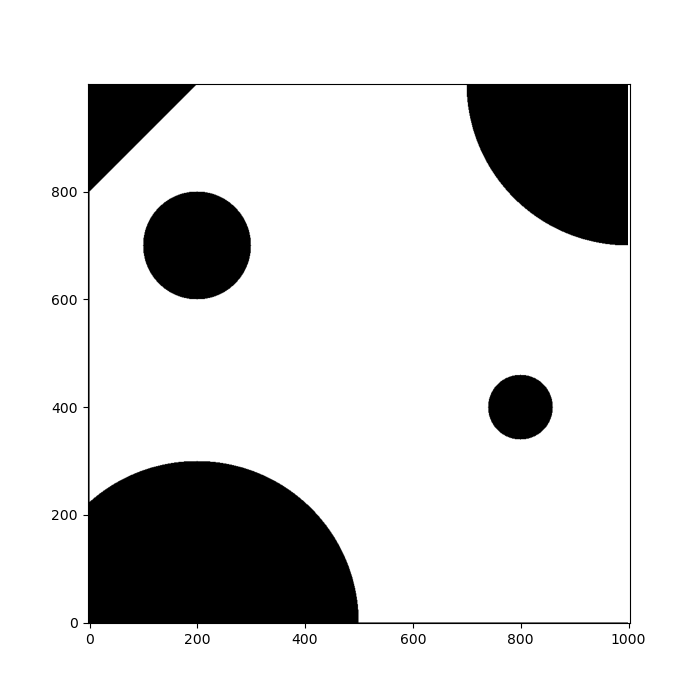
\includegraphics[width=10cm]{./przykladowa_mapa_pokoju.png}
		\caption{Przykładowa mapa pokoju}
		\label{przykladowa_mapa_pokoju}
	\end{center}
\end{figure}
\subsection{Samolot w locie}
Stan samolotu opisano tak samo jak stan robota w rozdziale \ref{robot_w_pomieszczeniu_desc}:
\begin{equation*}
	x = \{p_x,p_y,\theta,v\}
\end{equation*}
Mapa jest natomiast mapą wysokościową, w tym przypadku zdecydowano się na dwa warianty, pierwszy jest mapą fragmentu Wrocławia (przykład widoczny na rysunku \ref{przykladowa_mapa_wroclawia}), natomiast drugą wygenerowano jako szum, którego zmienność można kontrolować (przykład widoczny na rysunku \ref{przykladowa_mapa_szumu}).\\
O ile nie będzie napisane inaczej, samolot w lewym dolnym rogu mapy, miał prędkość 10 jednostek na iterację, i nie zmieniał orientacji $\theta=\frac{\pi}{4}$.
\begin{figure}
	\begin{center}
		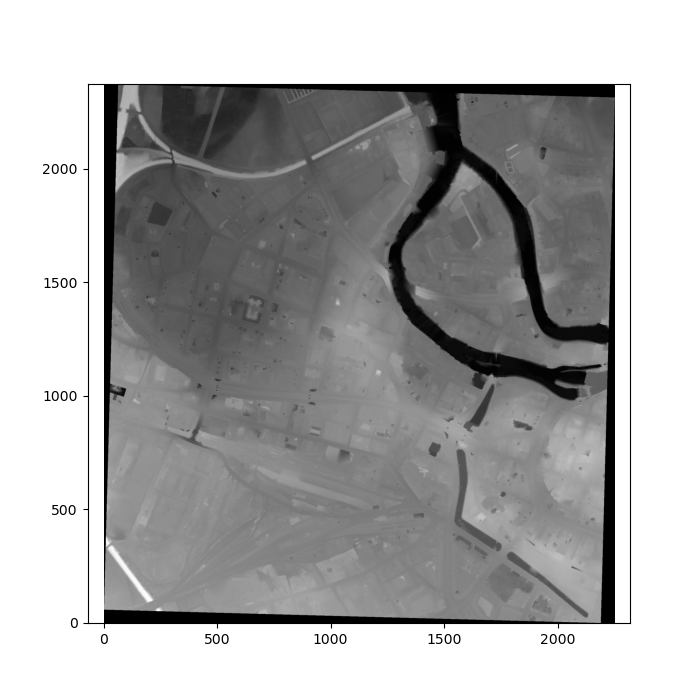
\includegraphics[width=10cm]{./przykladowa_mapa_wroclawia.png}
		\caption{Przykładowa mapa wysokościowa fragmentu Wrocławia}
		\label{przykladowa_mapa_wroclawia}
	\end{center}
\end{figure}
\begin{figure}
\begin{center}
	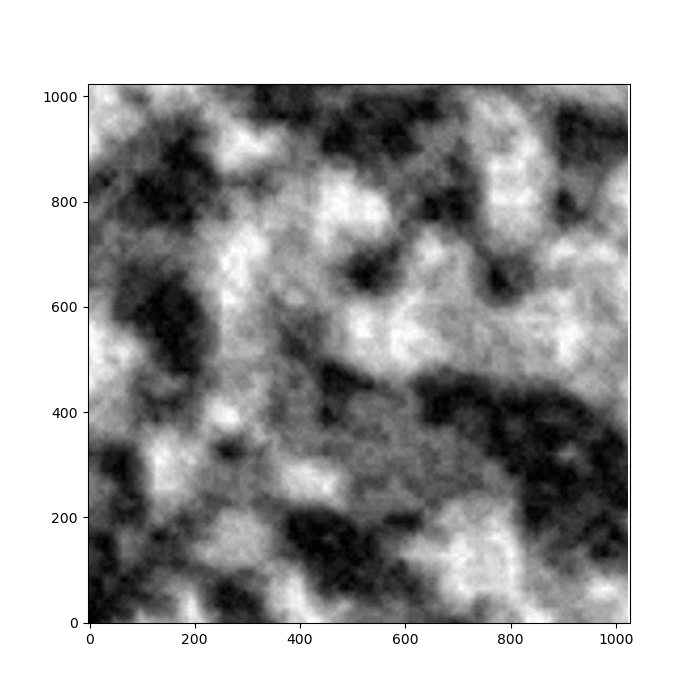
\includegraphics[width=10cm]{./przykladowa_mapa_szumu.png}
	\caption{Przykładowa mapa wysokościowa uzyskana z szumu}
	\label{przykladowa_mapa_szumu}
\end{center}
\end{figure}

\section{Badania poprawności działania}
W tym rozdziale zajęto się badaniami mającymi potwierdzić poprawne działanie zaimplementowanego rozwiązania. Na początku sprawdzono, jak zmiana generatora liczb losowych wpłynęła na wyniki, następnie sprawdzono, jak poradzi sobie algorytm przy braku punktów odniesienia, potem co się dzieje przy braku ewolucji systemu ($v=0$), a na koniec jak filtr radzi sobie z całkowicie losowymi pomiarami. Nie skupiano się no konkretnych wartościach liczbowych, jedynie wizualnie oceniano wyniki.

\subsection{Wpływ generatora}
Przebadano trzy generatory wbudowane w język C++: domyślny linear congruential generator(LCG) \cite{lcg_wiki}, Mersenne Twister \cite{mersenne_wiki} oraz wbudowany niedeterministyczny generator. Populacja cząstek wynosiła $N=1000$. Wyniki rysowano po 1, 11 i 21 iteracjach filtra(nr iteracji oznaczano jako $k$). Wyniki przedstawiono na rysunkach \ref{lcg_example}, \ref{mersenne_example}, \ref{device_example}. Jak widać dla wszystkich generatorów wyniki są niemal takie same, i zbiegają do faktycznego położenia robota. Ponieważ dla każdego generatora uzyskano poprawne wyniki, w dalszych badaniach korzystano z generatora LCG ponieważ jest najprostszy, i, co za tym idzie, najszybszy.

\begin{figure}
	\begin{center}
		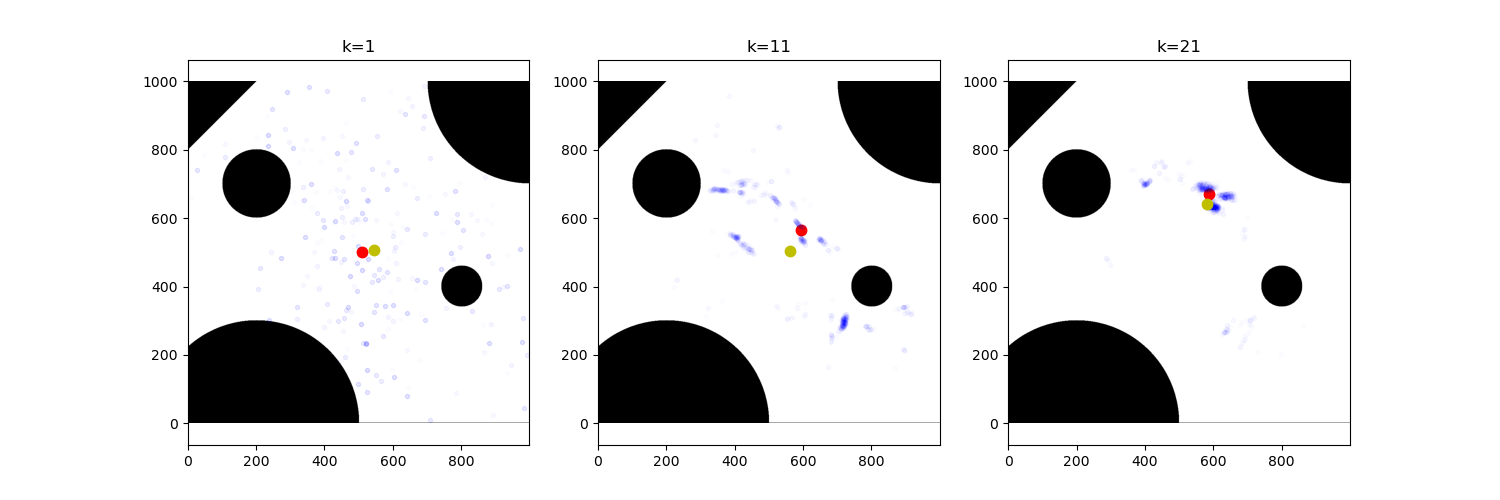
\includegraphics[width=15cm]{./lcg_example.png}
		\caption{Przykładowe wyniki dla generatora LCG}
		\label{lcg_example}
	\end{center}
\end{figure}

\begin{figure}
	\begin{center}
		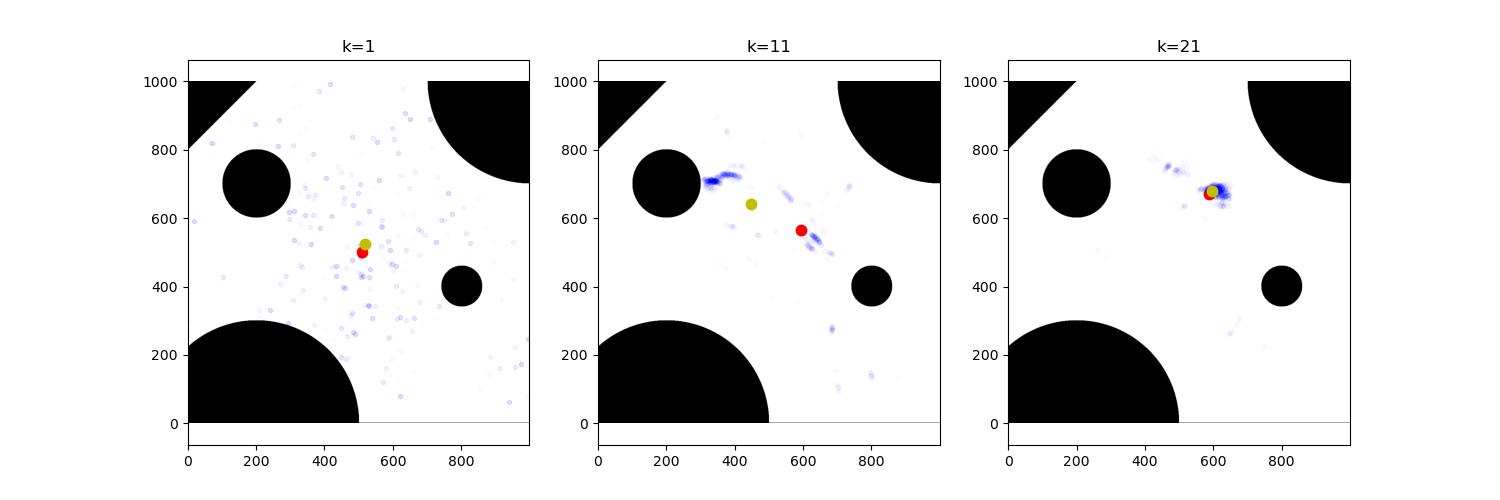
\includegraphics[width=15cm]{./mersenne_example.png}
		\caption{Przykładowe wyniki dla generatora Mersenne Twister}
		\label{mersenne_example}
	\end{center}
\end{figure}

\begin{figure}
\begin{center}
	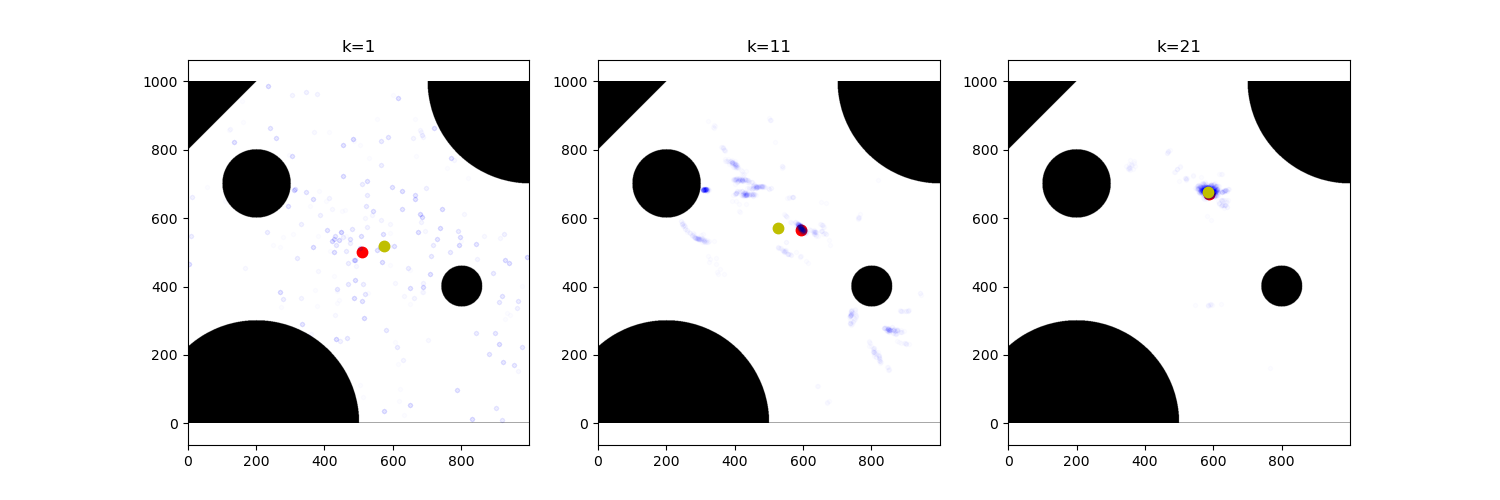
\includegraphics[width=15cm]{./device_example.png}
	\caption{Przykładowe wyniki dla niedeterministycznego generatora}
	\label{device_example}
\end{center}
\end{figure}


\subsection{Niejednoznaczna mapa}
W tym przypadku zbadano jak zachowa się filtr przy braku punktów odniesienia. W kwadratowym pokoju, powinno to spowodować pojawienie się czterech równie prawdopodobnych pozycji. Jak widać przewidywania potwierdziły się na rysunku \ref{no_pivot}. Na rysunku \ref{one_pivot} przedstawiono sytuację, gdy mapa dopuszcza dwie możliwe pozycja. Badania przeprowadzono przy populacji $N=10000$ cząstek.

\begin{figure}
	\begin{center}
		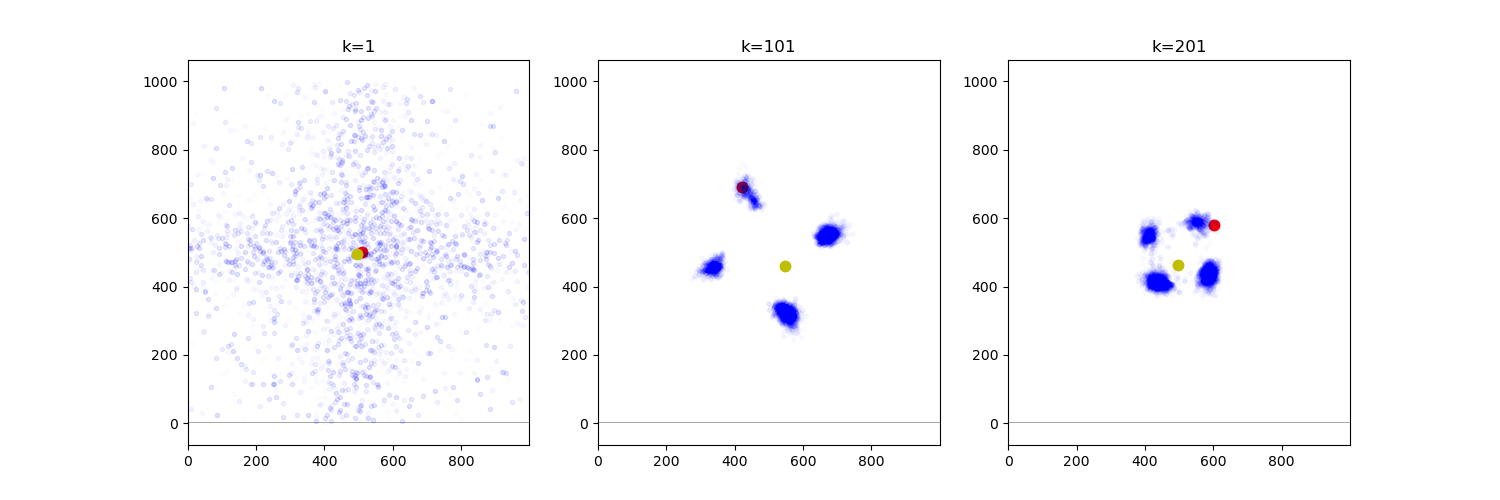
\includegraphics[width=15cm]{./no_pivot.png}
		\caption{Przykładowe wyniki przy braku punktu odniesienia}
		\label{no_pivot}
	\end{center}
\end{figure}

\begin{figure}
	\begin{center}
		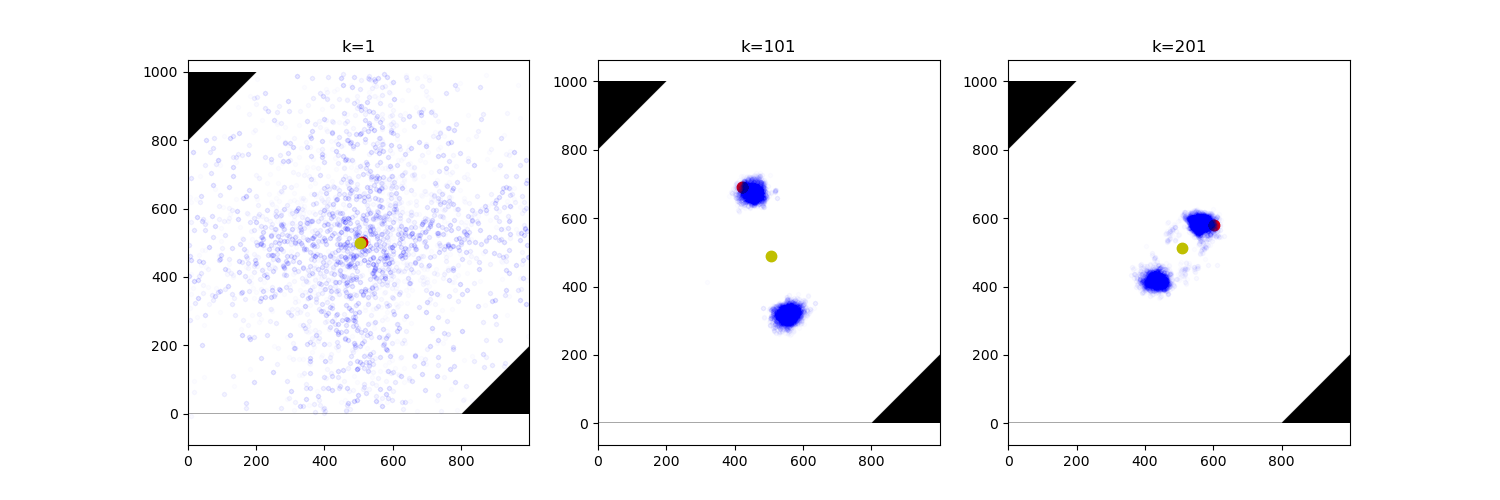
\includegraphics[width=15cm]{./one_pivot.png}
		\caption{Przykładowe wyniki przy dwóch możliwych położeniach}
		\label{one_pivot}
	\end{center}
\end{figure}

\subsection{Brak ewolucji systemu}
Tutaj Zbadano, co się dzieje, gdy system nie ewoluuje. Spodziewano się, pojawią się izohipsy, przynajmniej na początku, nim populacja nie stanie się zbyt zdegenerowana. Badania przeprowadzono dla populacji o rozmiarze $N=100000$. Jak widać na rysunkach \ref{stationary} i \ref{stationary_plane} przewidywania się spełniły, dodatkowo dla rysunku \ref{stationary_plane} dobrze widać pojawianie się degeneracji.

\begin{figure}
	\begin{center}
		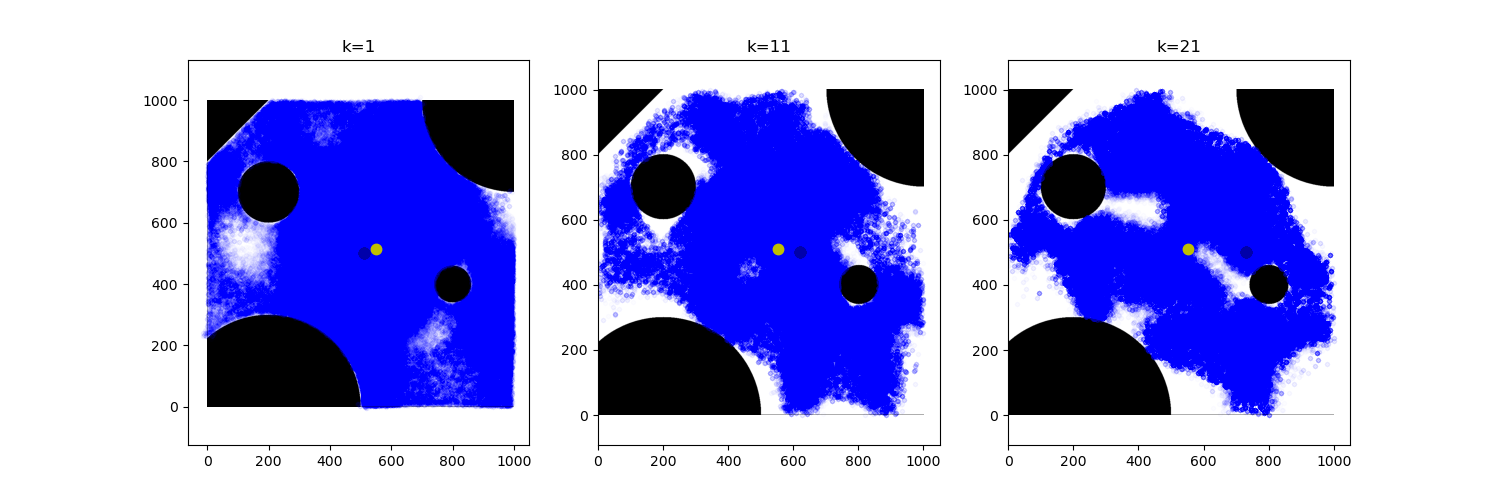
\includegraphics[width=15cm]{./stationary.png}
		\caption{Przykładowe wyniki przy braku ewolucji systemu, dla robota w pokoju}
		\label{stationary}
	\end{center}
\end{figure}

\begin{figure}
\begin{center}
	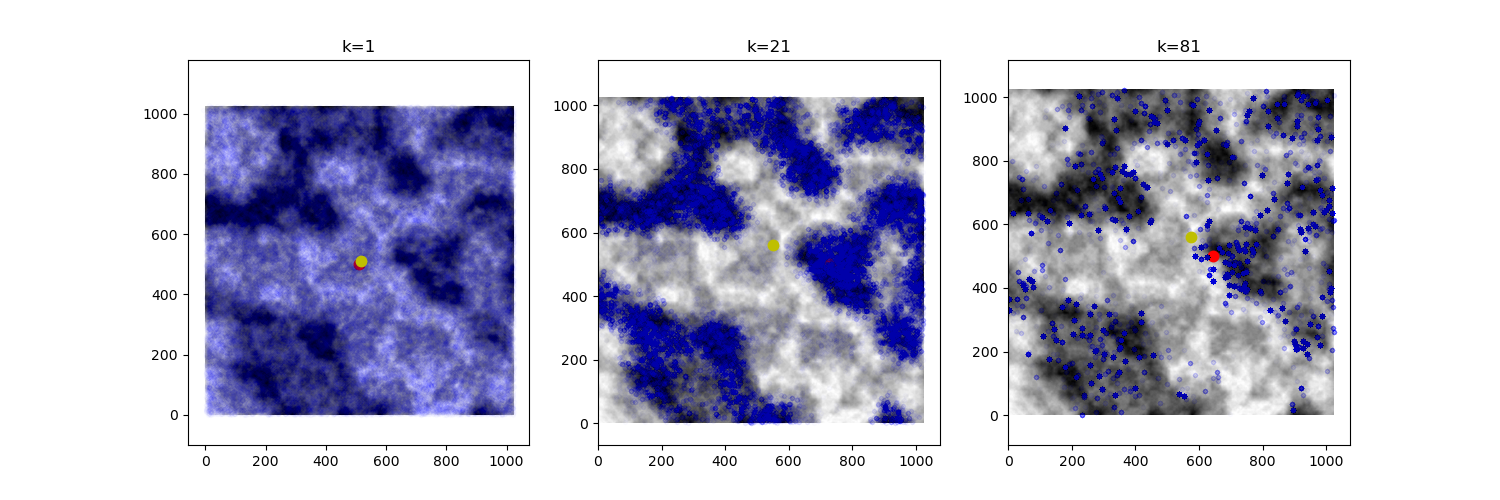
\includegraphics[width=15cm]{./stationary_plane.png}
	\caption{Przykładowe wyniki przy braku ewolucji systemu, dla samolotu}
	\label{stationary_plane}
\end{center}
\end{figure}

\subsection{Pomiary bez związku}
powinien pozostać jednostajny szum

\section{Wpływ sposobu estymowania położenia}
\section{Wpływ funkcji określającej błąd pomiaru}
\section{Wpływ liczby cząstek}
\section{Wpływ metody próbkowania}
\section{Skuteczność w poprawianiu błędnie określonego położenia}
\section{Wpływ szumu}
\section{Wpływ różnorodności terenu}
\section{Rozkład p przy dryfie - chodzi o genetyczne}


	\chapter{Wnioski}
\begin{itemize}
	\item 
\end{itemize}
\section{Podsumawanie}
co w kolejnych rozdziałach

\chapter{Kierunki przyszłych badań}
\begin{itemize}
	\item Zrezygnowanie z implementacji C++ na rzecz całkowitego przejścia na Python, z wykorzystaniem na przykład pakietu Numba \cite{numba}. Poza przyspieszeniem porównywalnym z C++, pozwoliło by na przykład na poszerzanie kodu o obliczenia na karcie graficznej. Dzięki temu, można by spróbować rozwiązać problem robota w pokoju, wykorzystując Box Particle Filter.
	\item zamiast avg, np klasteryzacja?
\end{itemize}
	
	\newpage
	\listoffigures
%	\newpage
%	\listoftables
	
	\bibliographystyle{plabbrv}
	\bibliography{biblio}
\end{document}